
\section{Results and discussion}
\label{sec:result}

In this section, we present some computational results of the proposed approach. Our approach offers a global stiffness design of interior structure with the input surface mesh and the amount of material allowed. Our algorithm is applied to a variety of objects that would be applied with different load distributions in regular use like American football, toys and models. We first verify the optimization results of our formulation with the analysis framework in Sec.~\ref{subsec:mechanics}, and then verify the final results of the whole framework which are generated based on the optimized frame structures. Different from verifying the result of optimization under given load, our global stiffness optimization result is difficult to test in real physical experiment but thanks to the advance of FEM technique, we examed our results based on a FEM-based computational framework that can be considered as a good simulation of physical experiment, which will be discussed later. 

\noindent\textbf{Criteria} With a $10N$ load is applied, two criteria are discussed here: \textit{Average} deformation and \textit{Maximum} deformation. $4000$ random load distribution cases are applied and the \textit{Average} is the mean value of the norm of the $4000$ deformation led by corresponding load distributions. \textit{Maximum} is obtained by applying the load that leads to the maximum norm of deformation: on frame structure, the load distribution is given by the inner optimization of our formulation, i.e., $\max\limits_{F \mbox{ satisfying }  (\ref{cond-for-F}) } \frac{{(\hat{K}^{-1}F)}^T(\hat{K}^{-1}F)}{{F}^TF}$; on the final object, the load distribution is given by the result of \cite{zhou:2013}. In our experiment, the amount of material use is set to be the $20\%$ of the solid volume of the input object. A better global stiffness property means the less value these two criteria are. 

All the experiments were conducted on a PC with a 2.8GHZ Core CPU and 8GB RAM, running Linux OS.

To verify the global stiffness property of our optimized frame structure, we compare it and the initial structure with uniform beam radii. The uniform radii is set to make the control structure have the same volume as our result. In Fig.~\ref{fig_frame_hand_case}, two certain cases of the hand model is presented where warmer color refers to a larger value of deformation and cooler color refers to a smaller value of deformation. For all the tested models, the map of the \textit{Maximum} deformation is illustrated in Fig.~\ref{fig_frame_max}. With the statistic data in Table~\ref{table_frame}, our proposed formulation is proved to be able to optimize the global stiffness of a given initial frame structure.


\begin{figure}[h]
  \centering
  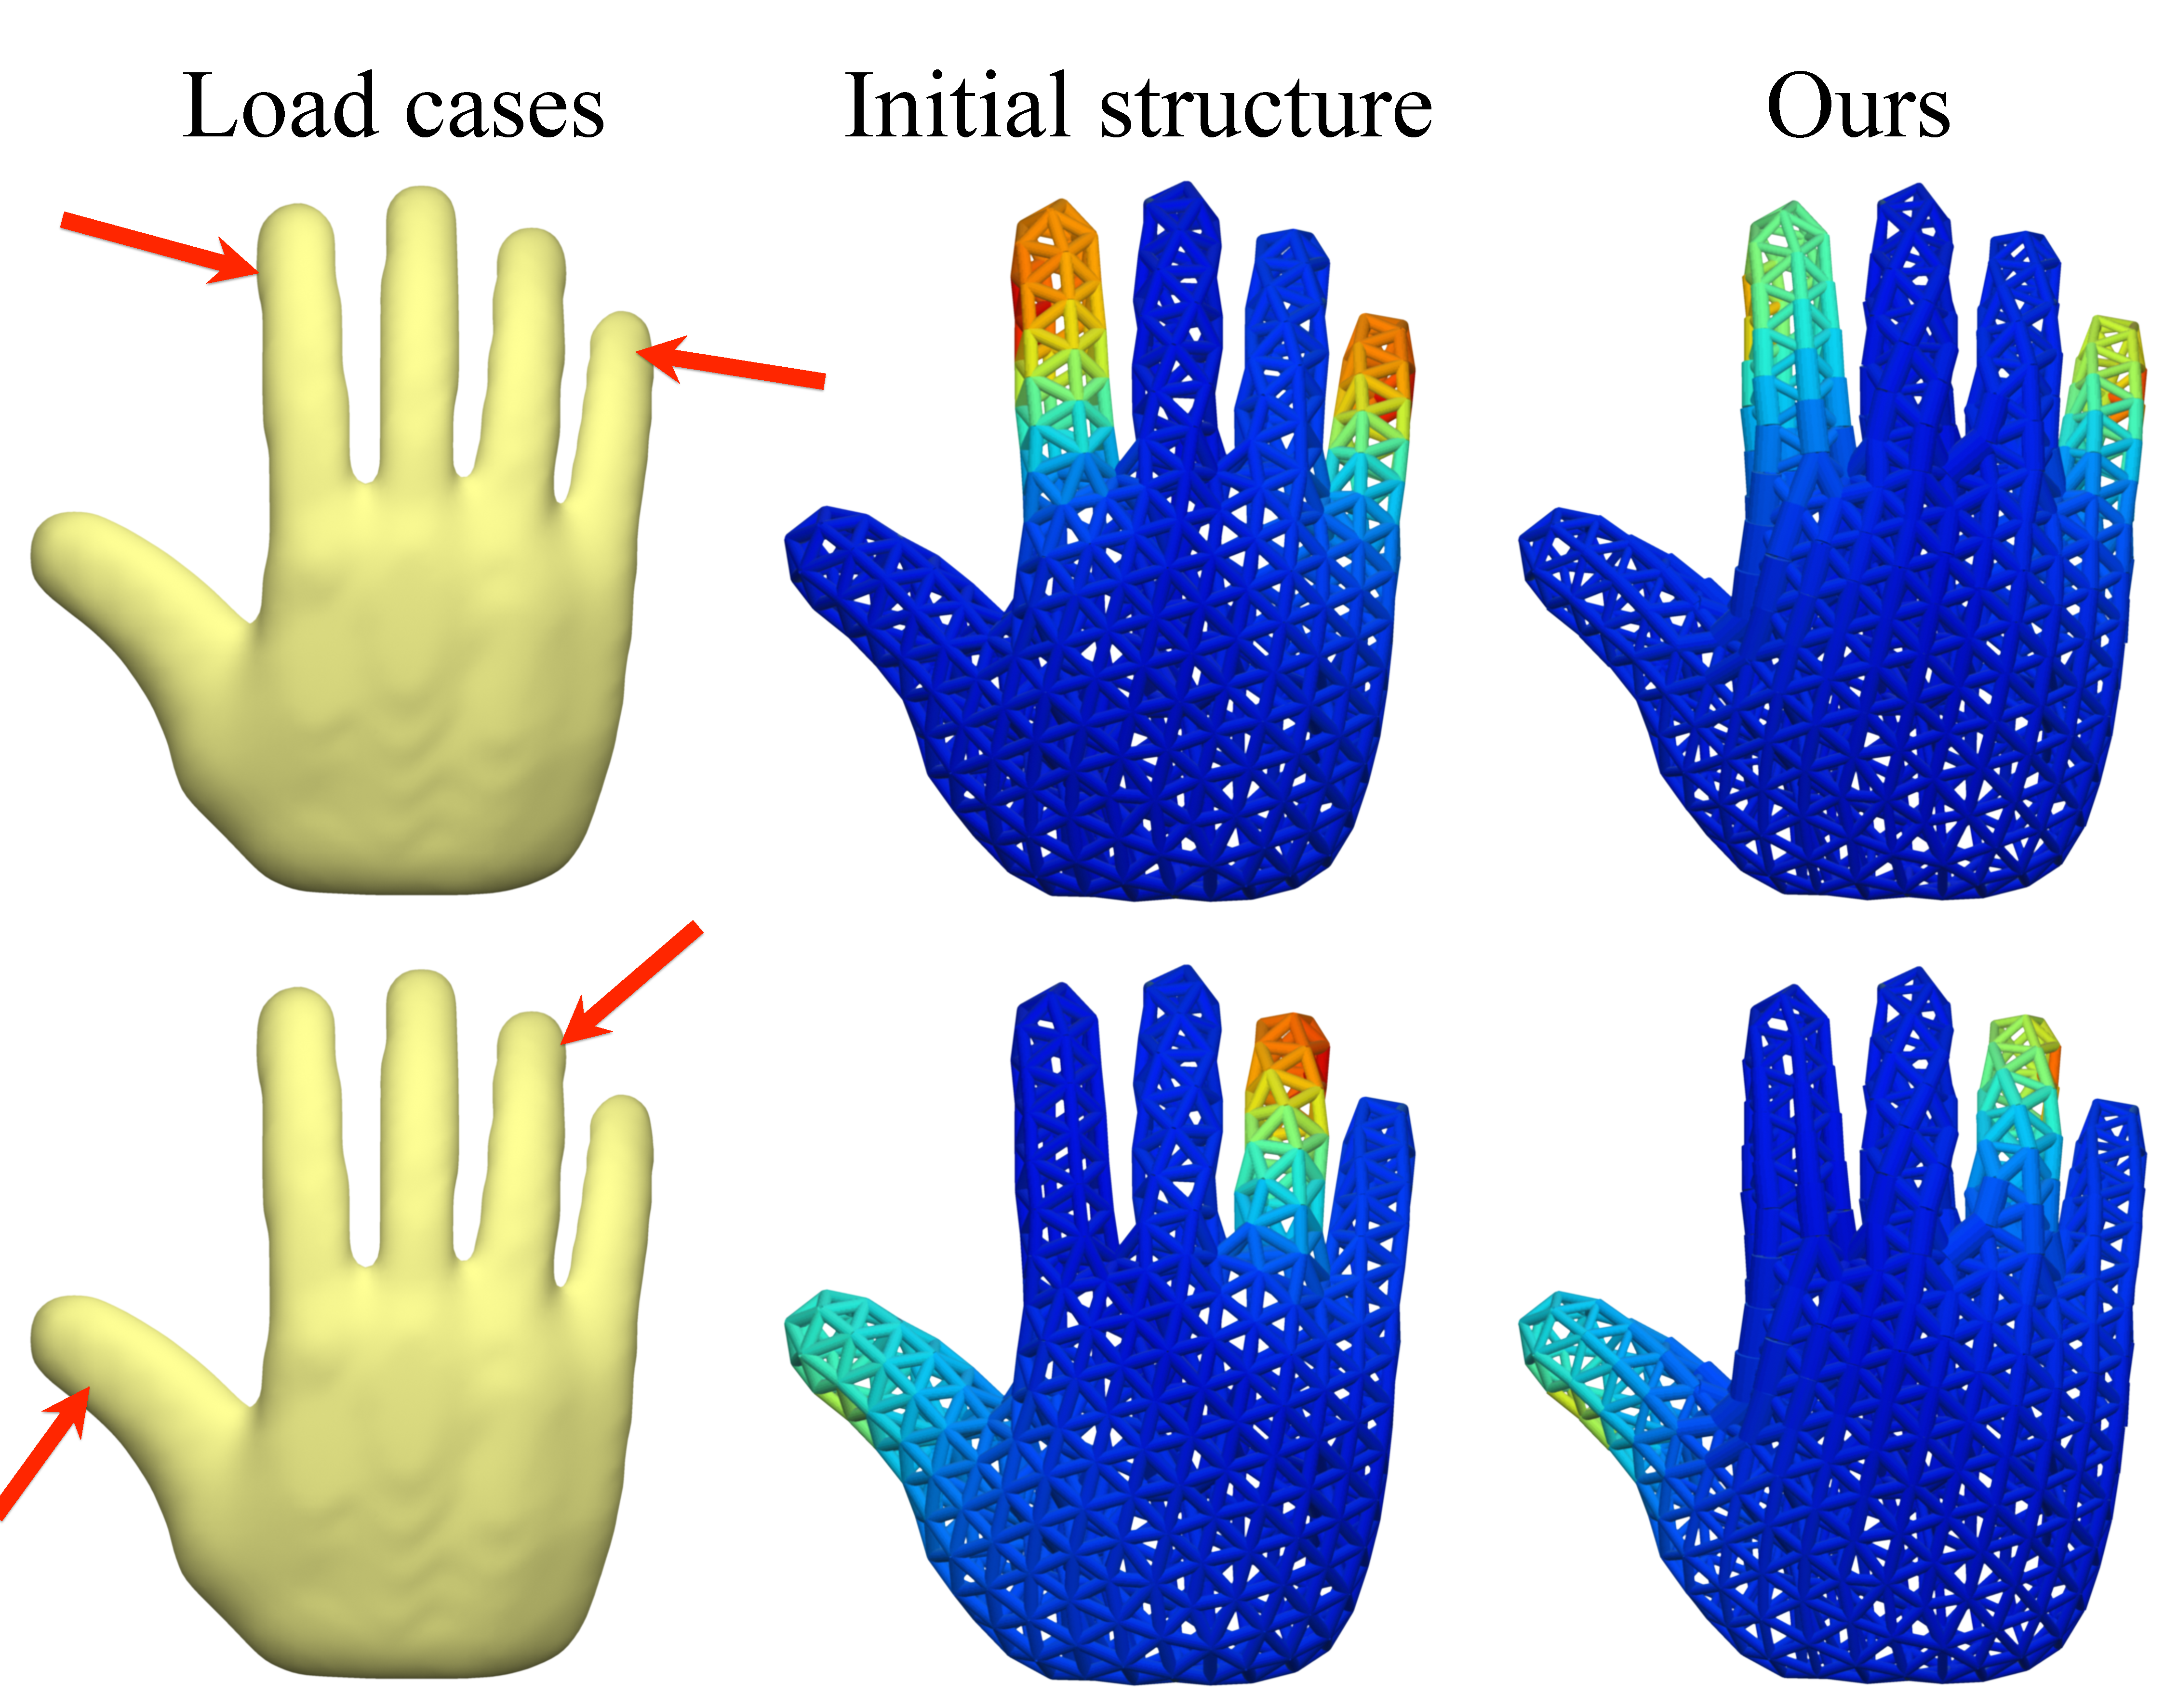
\includegraphics[width=0.5\linewidth]{Figures/hand/hand.pdf}
  \caption{\label{fig_frame_hand_case} Deformation distribution of two certain load distribution cases (top and bottom row) on the initial structure and our optimized structure of hand model. The red arrows shown on the model indicate that the deformation is simulated under the certain pair of forces. The initial structure we tested have the same volume with our result. Warmer color refers to a larger value of deformation and cooler color refers to a smaller value of deformation. It is obvious that our result performs better in these two selected cases.}
\end{figure}

\begin{figure*}[t]

  \centering
            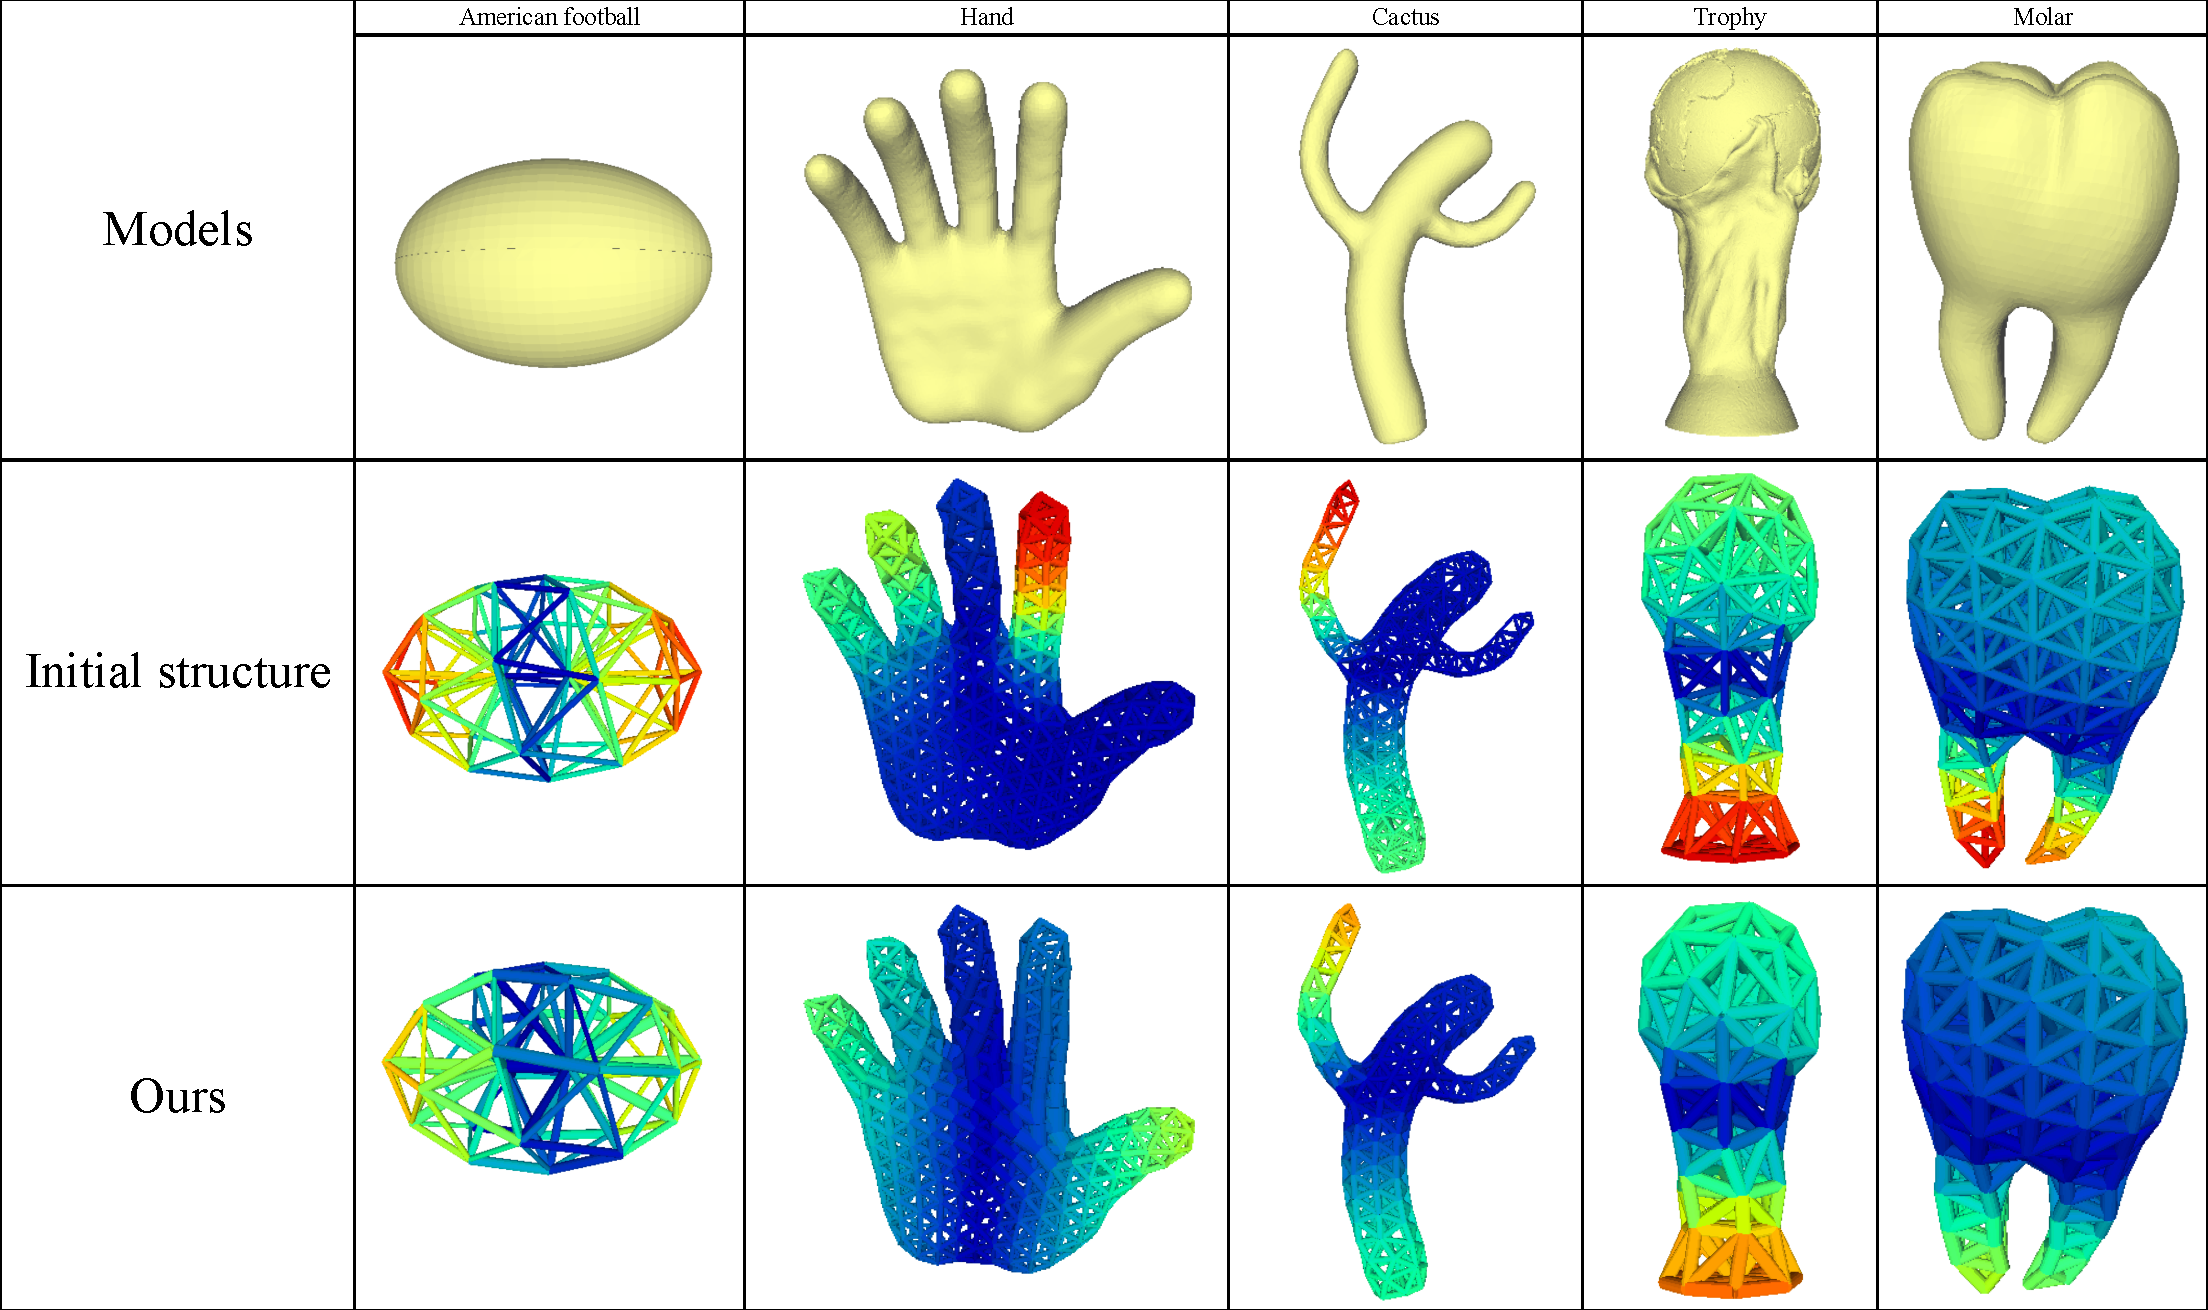
\includegraphics[width=.85\linewidth]{Figures/fig4/fig4.pdf}
    
\caption{\label{fig_frame_max}
  Maximum deformation distribution case for test frame structures.
            Top: Input model; Middle: distribution map of initial structure; Bottom: distribution map of our optimized structure.
            The magnitude of maximum deformation on our resulting structure is much smaller than that on the uniform initial frame structure. Note that, for example in the hand model, the worst case is changing during our optimization of the frame structures}
\end{figure*}

\begin{table}[htb]
\caption{\label{table_frame}Statistics of tests for frame structure. Mean values of 4000 records of deformation (in mm) for each model are listed. The maximum deformation value for each model is also listed. First two rows are the results of uniform frame and the last two rows are our results .}
\centering
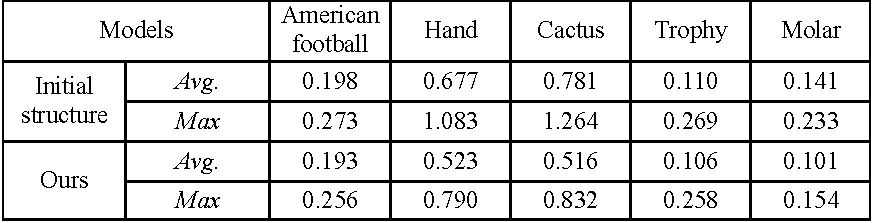
\includegraphics[width=0.5\linewidth]{Tables/table1}
\end{table}

\noindent\textbf{Physical experiment simulation} For examing the final object generated based on the optimized frame structure, FEM-based computation framework need to be adapted. For an elastic body $\Omega$, the stionary state of objects under forces can be described by the linear elasticity problem,
\begin{align}\label{eq:linear-elasticity}
     -\mbox{div}(\sigma(\epsilon(u))) & = f, \quad in\ \Omega \notag \\
                             u & = 0, \quad on\ \Gamma_D \\
          \sigma(\epsilon(u))\cdot n & = g, \quad on\ \Gamma_N. \notag
\end{align}
In this problem, $u$ is displacement, $\epsilon(u)=1/2(\nabla u+\nabla u^T)$ is the strain,
and $\sigma(\epsilon)=2\mu\epsilon+\gamma(\mathrm{tr}(\epsilon))I$ is the stress.
The quantities $\gamma$ and $\mu$ are the Lame moduli of the material. Such a problem can be solved by using FEMs. In our experiment, the FEM computation is executed by using DOLFIN~\cite{DOLFIN}.

We compare our results and uniform hollowing solution. In Fig.~\ref{fig_obj_hand}, we show the comparsion of the same cases as shown in Fig.~\ref{fig_frame_hand_case} for the hand model. General statistic data is shown in Table~\ref{table_obj}. We also compare our reuslt with \cite{Lu:2014}. We generate a global stiffness molar model which has the same volume with the molar example provided by this work as shown in Fig.~\ref{fig_cmp_btl}. 
%Two certain cases are shown in Fig.~\ref{fig_comp_btl}. 
The simluated results show that ours are more suitable under unknown load cases. 

\begin{figure}[h]
  \centering
  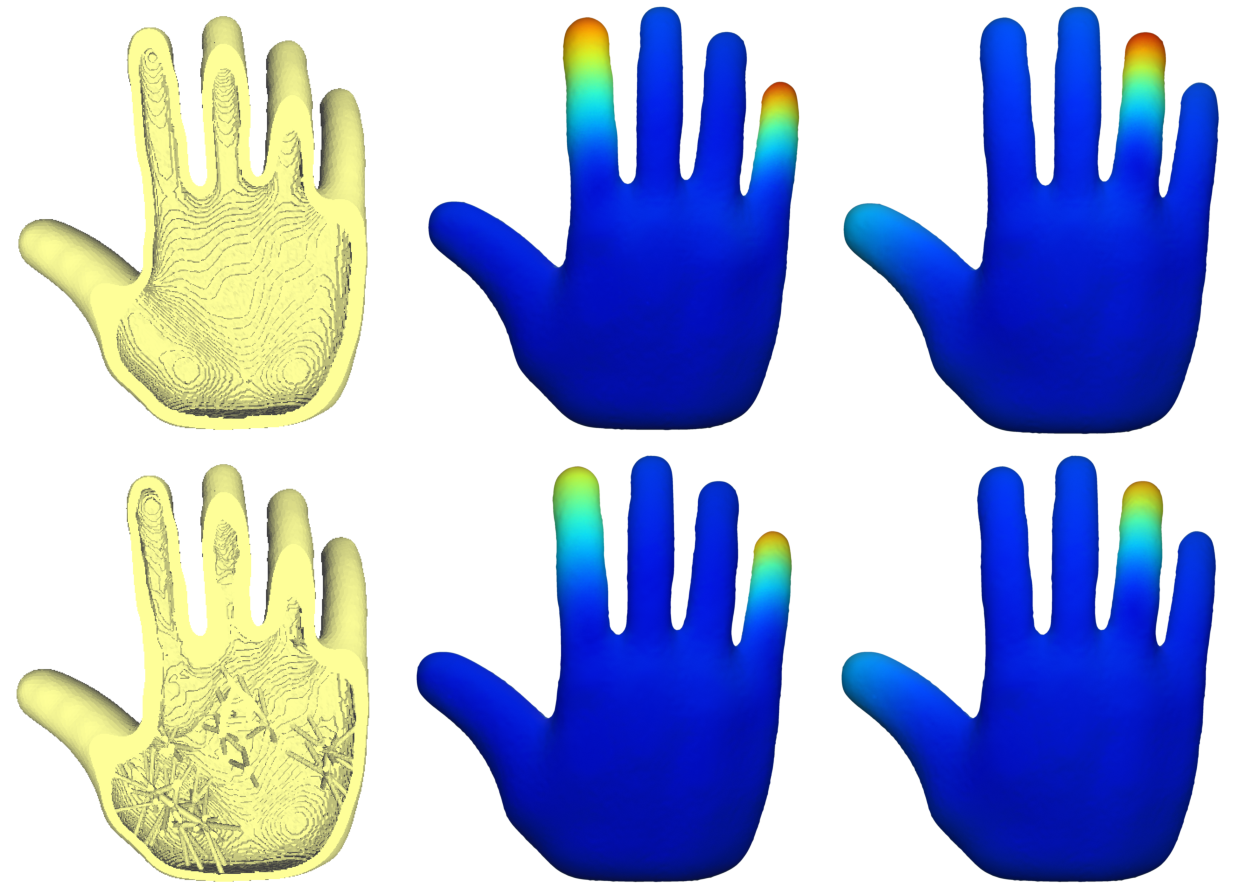
\includegraphics[width=0.5\linewidth]{Figures/hand/fig_obj_hand.pdf}
  \caption{\label{fig_obj_hand} Deformation distribution of the two load distribution cases (same as the cases shown in Fig.~\ref{fig_frame_hand_case}) on the uniform hollowing result (top) and our optimal result (bottom) of hand model. The first colume is the sectional view. The load is acted as pinching the forefinger and the little finger for the second colume and pinching the thumb and the third finger for the last colume. Two objects we tested have the same volume. It can be observe that the final object generated by our proposed postpocessing can sucessfully inherit the mechanical property and preforms better.}
\end{figure}

\begin{table}[htb]
\caption{\label{table_obj}Statistics of the simulation tests for object. Mean values of 4000 records of deformation (in mm) for each model are listed. The maximum deformation value for each model is also listed. First two rows are the results of uniform hollowing solution and the last two rows are our results .}
\centering
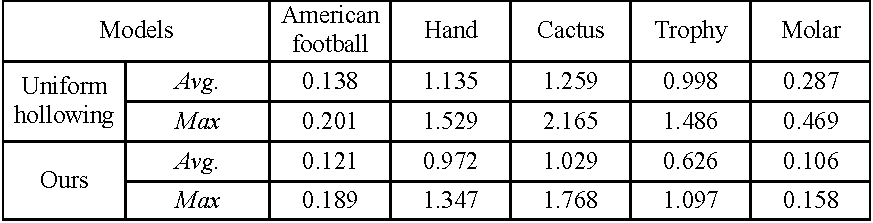
\includegraphics[width=0.5\linewidth]{Tables/table2}
\end{table}

\begin{figure}[h]
  \centering
  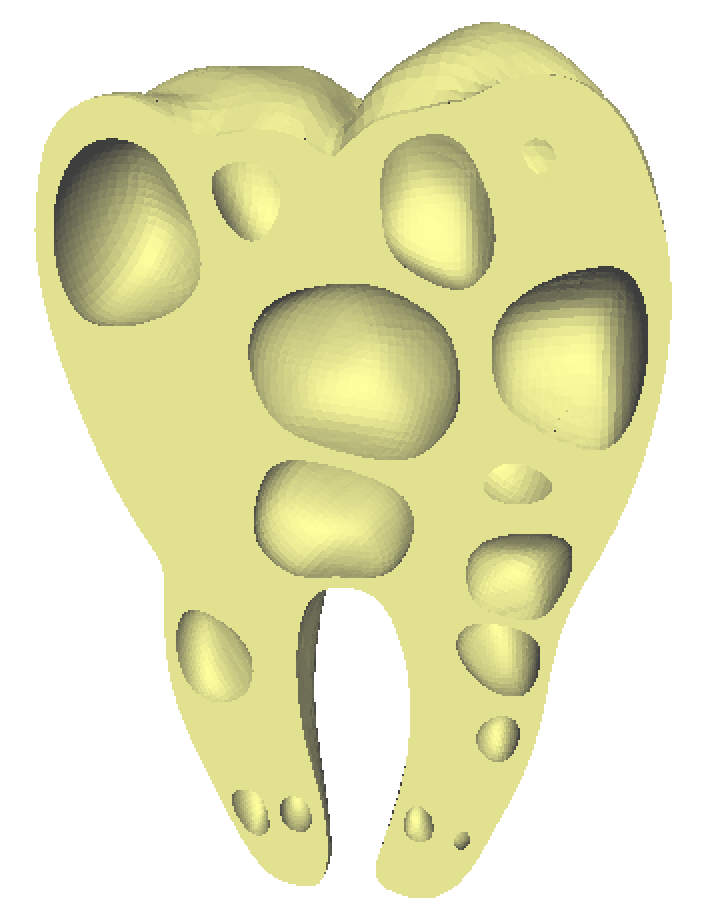
\includegraphics[width=0.2\linewidth]{Figures/molar_cmp/m2}
  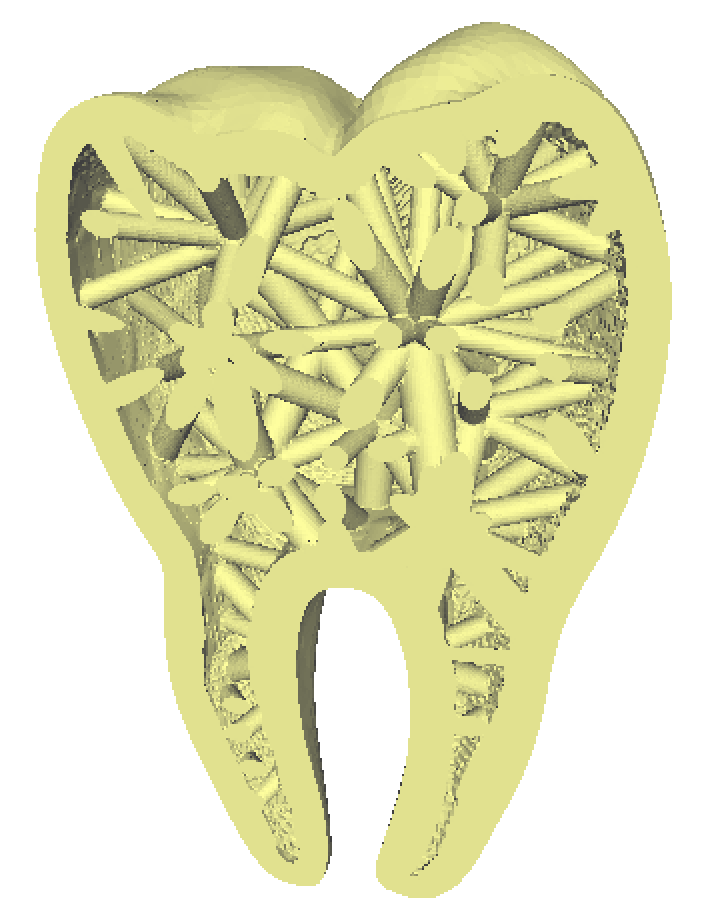
\includegraphics[width=0.2\linewidth]{Figures/molar_cmp/m1}

  \caption{\label{fig_cmp_btl} We compare our result with \cite{Lu:2014}. The left one is provided by \cite{Lu:2014} and the right one is ours. Two result objects have the same volume and the (Avg., Max) deformation is (0.125,0.197) and (0.106,0.158), respectively.}
\end{figure}

\begin{figure}[!h]
  \centering
  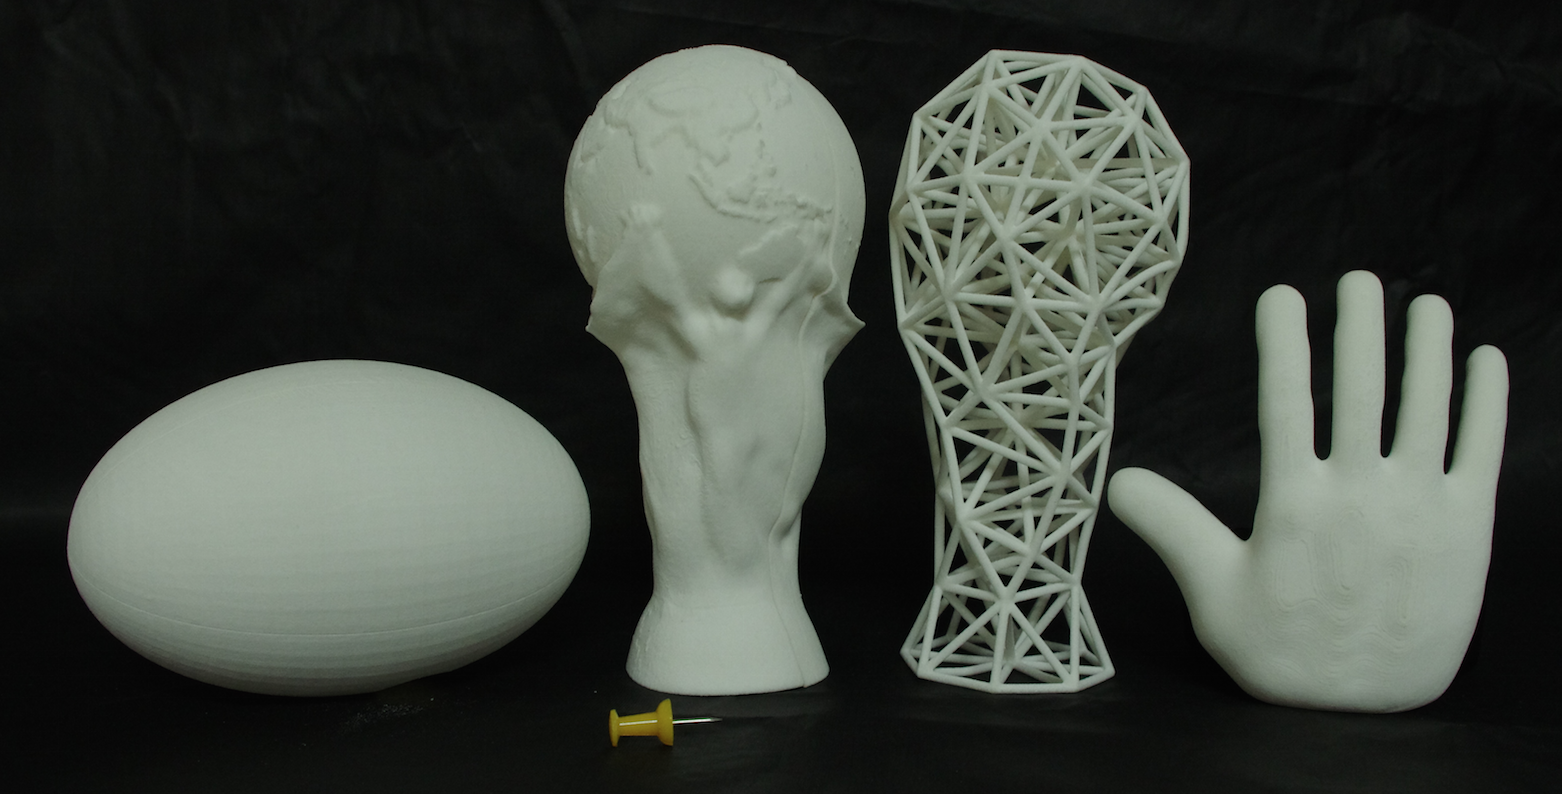
\includegraphics[width=0.5\linewidth]{Figures/results/1}
  \caption{\label{fig_all} We fabricate the final results for some models.}
\end{figure}

Our saddle point optimization problem can be solved very efficiently. All examples appear in this paper are optimized within 20mins.






